%!TEX root =  main.tex


\begin{figure*}[!ht]
    \centering
    \setlength{\tabcolsep}{1pt} 
    \resizebox{0.99\linewidth}{!}{
    \begin{tabular}{ccccc}
        & \hspace{8mm}\textbf{Arena} & \hspace{8mm}\textbf{ShareGPT} & \hspace{8mm}\textbf{Spec-Bench}  & \hspace{8mm}\textbf{Tough}\\
               
        \rotatebox{90}{\parbox{3.5cm}{\centering \hspace{8mm}\textbf{Qwen3~32B-0.6B}}} &
        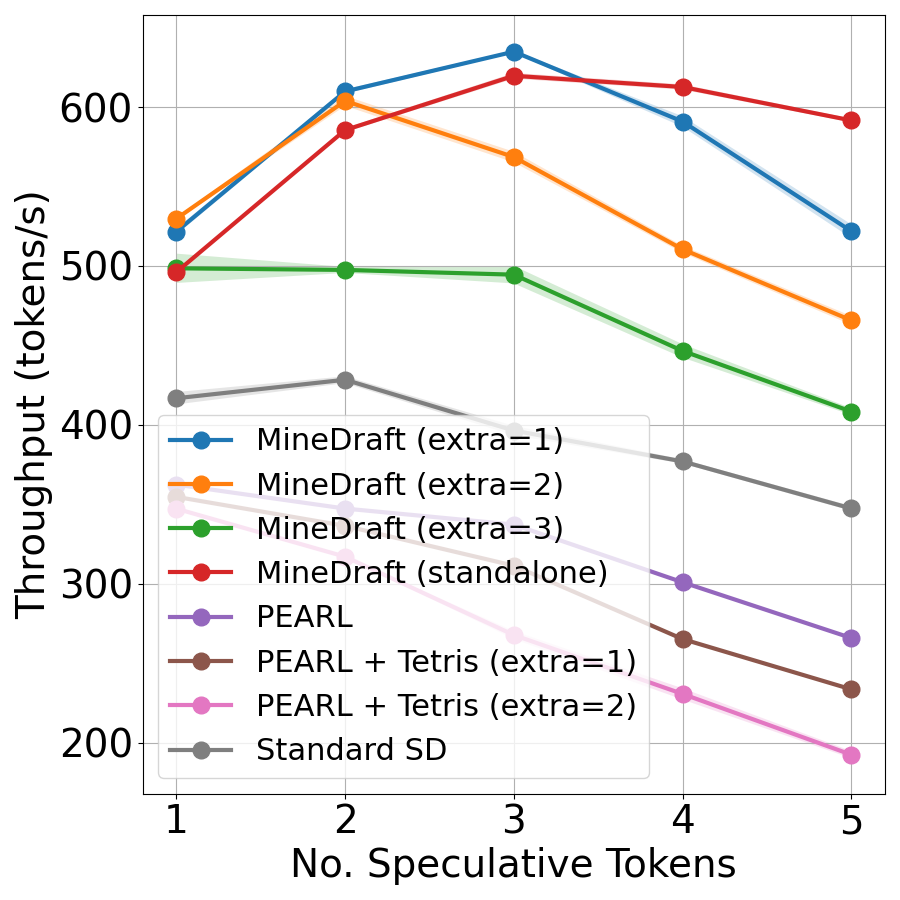
\includegraphics[width=0.23\linewidth]{results/Arena_Qwen3-32B_Qwen3-0_6B_1000_bs16_100pct_gen_throughput.png} &
        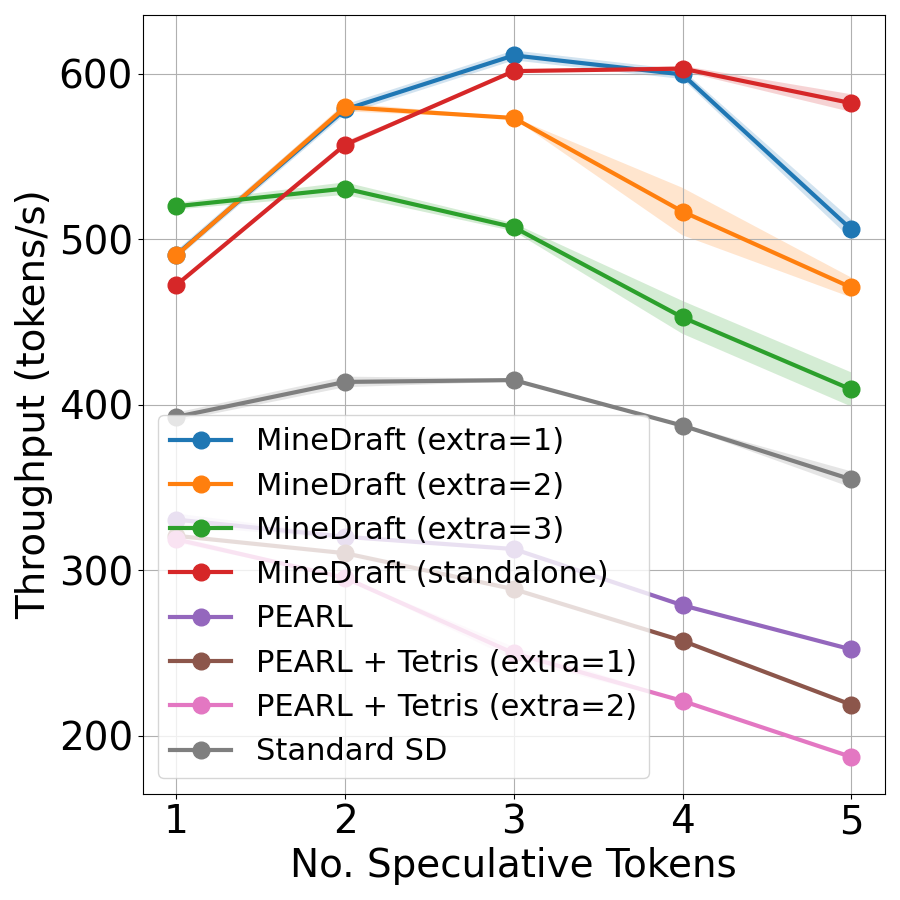
\includegraphics[width=0.23\linewidth]{results/ShareGPT_Qwen3-32B_Qwen3-0_6B_1000_bs16_100pct_gen_throughput.png} &
        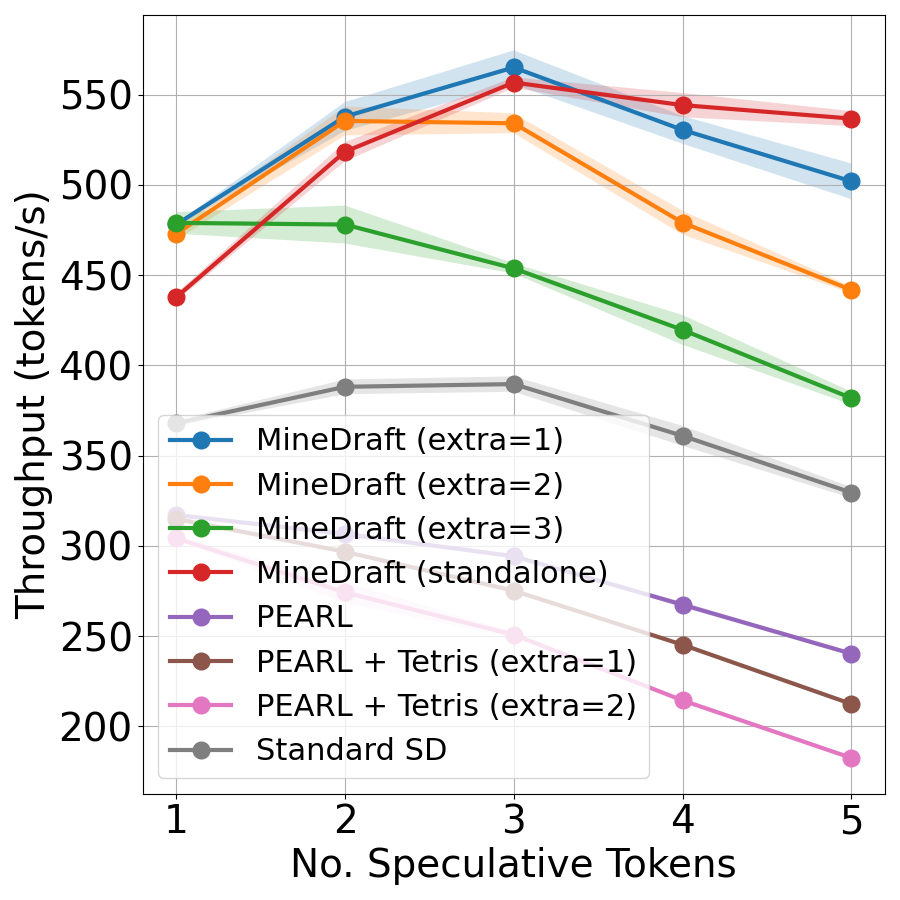
\includegraphics[width=0.23\linewidth]{results/Spec-Bench_Qwen3-32B_Qwen3-0_6B_161_bs16_100pct_gen_throughput.png} &
        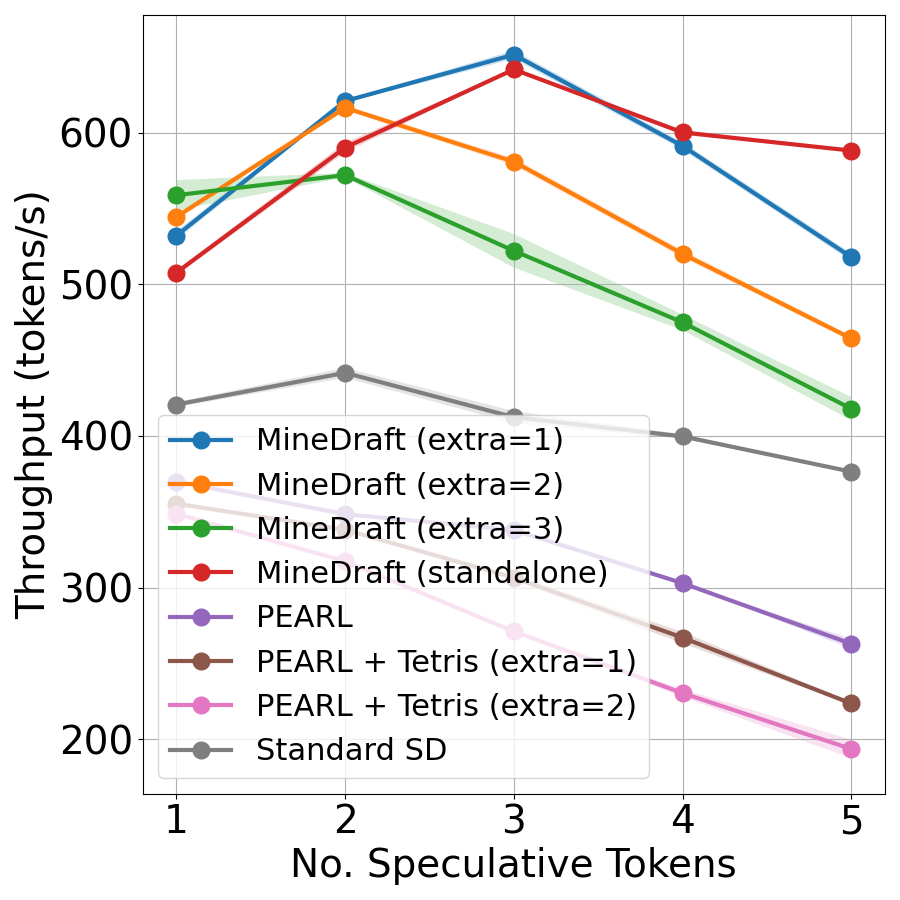
\includegraphics[width=0.23\linewidth]{results/Tough_Qwen3-32B_Qwen3-0_6B_1000_bs16_100pct_gen_throughput.png} \\
        & \hspace{2mm}(i) \hspace{2mm} $\uparrow$ 42.36\%, $\Delta$ 70.32\% &
        \hspace{2mm}(j) \hspace{2mm} $\uparrow$ 47.28\%, $\Delta$ 64.05\% &
        \hspace{2mm}(k) \hspace{2mm} $\uparrow$ 45.02\%, $\Delta$ 62.87\% &
        \hspace{2mm}(l) \hspace{2mm} $\uparrow$ 40.59\%, $\Delta$ 57.95\% \\

        \rotatebox{90}{\parbox{3.5cm}{\centering \hspace{8mm}\textbf{Qwen3~32B-1.7B}}} &
        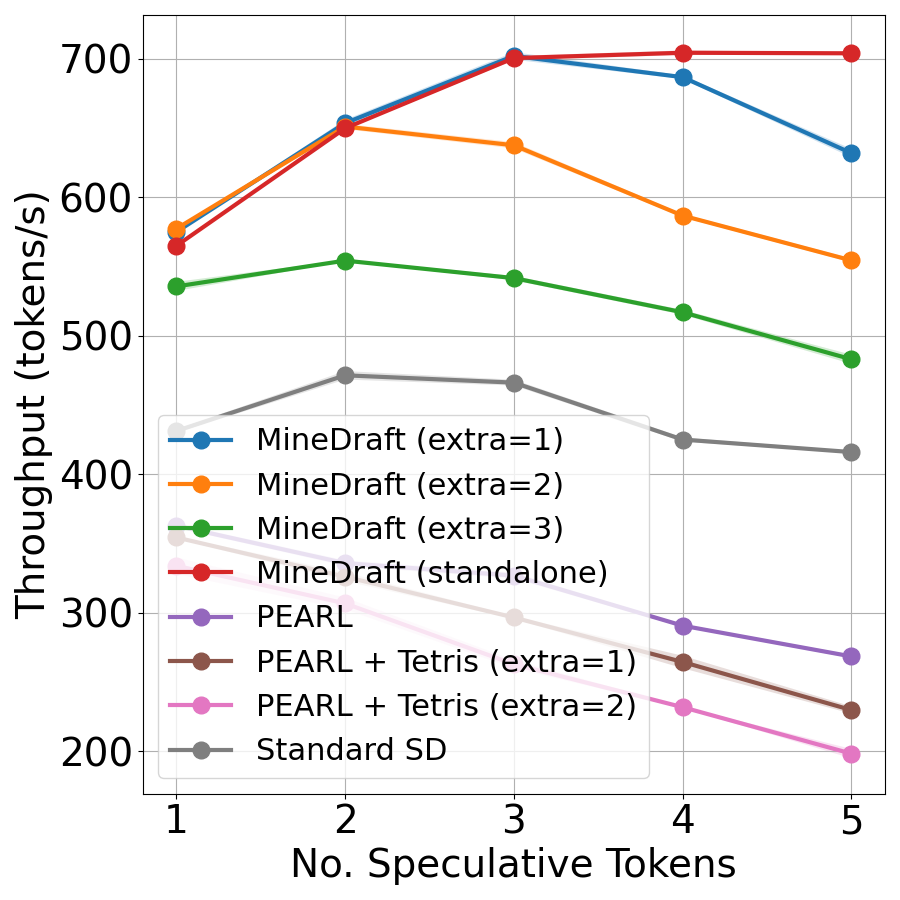
\includegraphics[width=0.23\linewidth]{results/Arena_Qwen3-32B_Qwen3-1_7B_1000_bs16_100pct_gen_throughput.png} &
        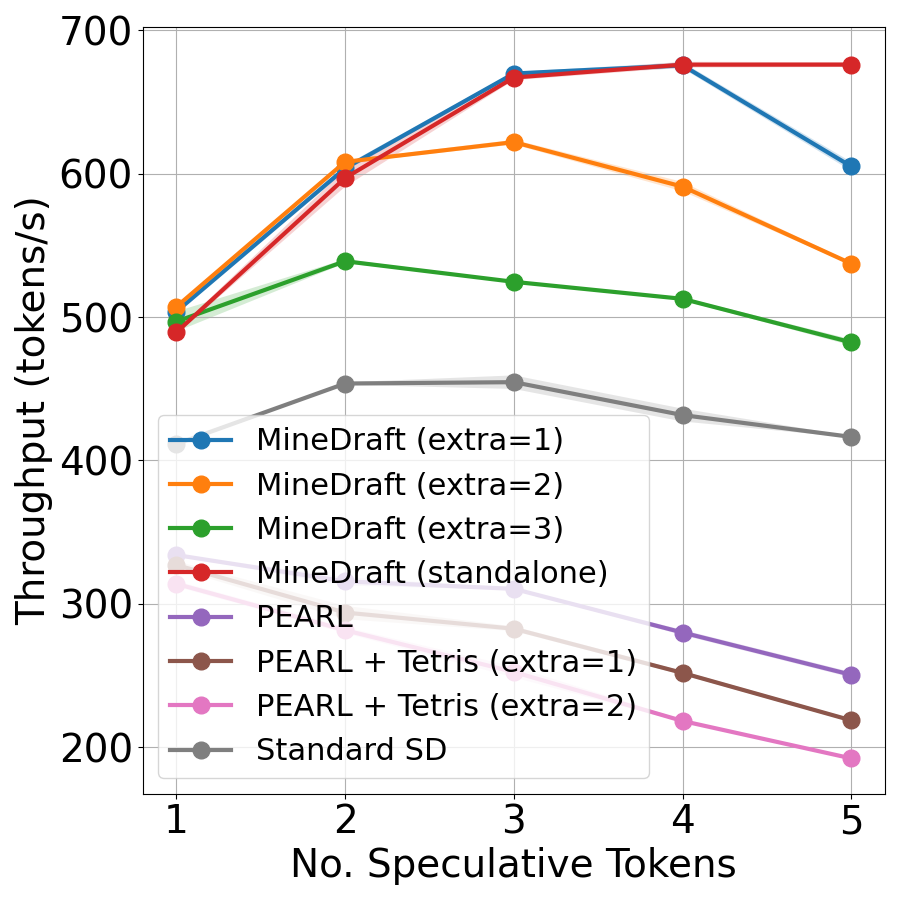
\includegraphics[width=0.23\linewidth]{results/ShareGPT_Qwen3-32B_Qwen3-1_7B_1000_bs16_100pct_gen_throughput.png} &
        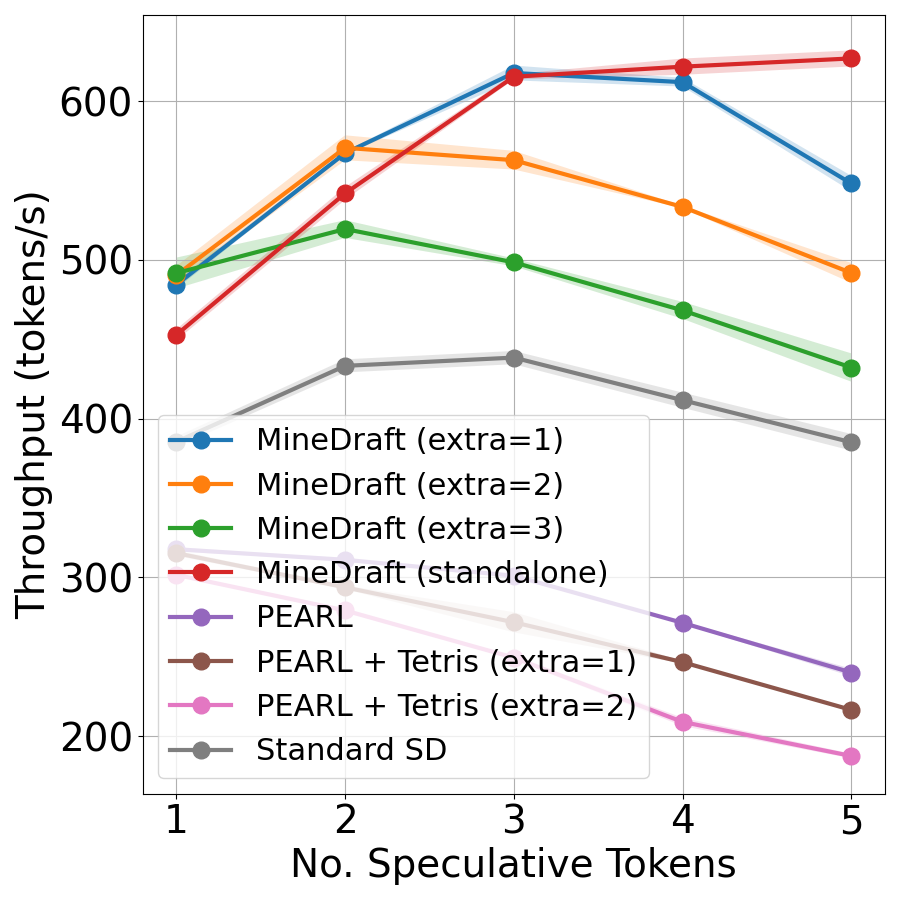
\includegraphics[width=0.23\linewidth]{results/Spec-Bench_Qwen3-32B_Qwen3-1_7B_161_bs16_100pct_gen_throughput.png} &
        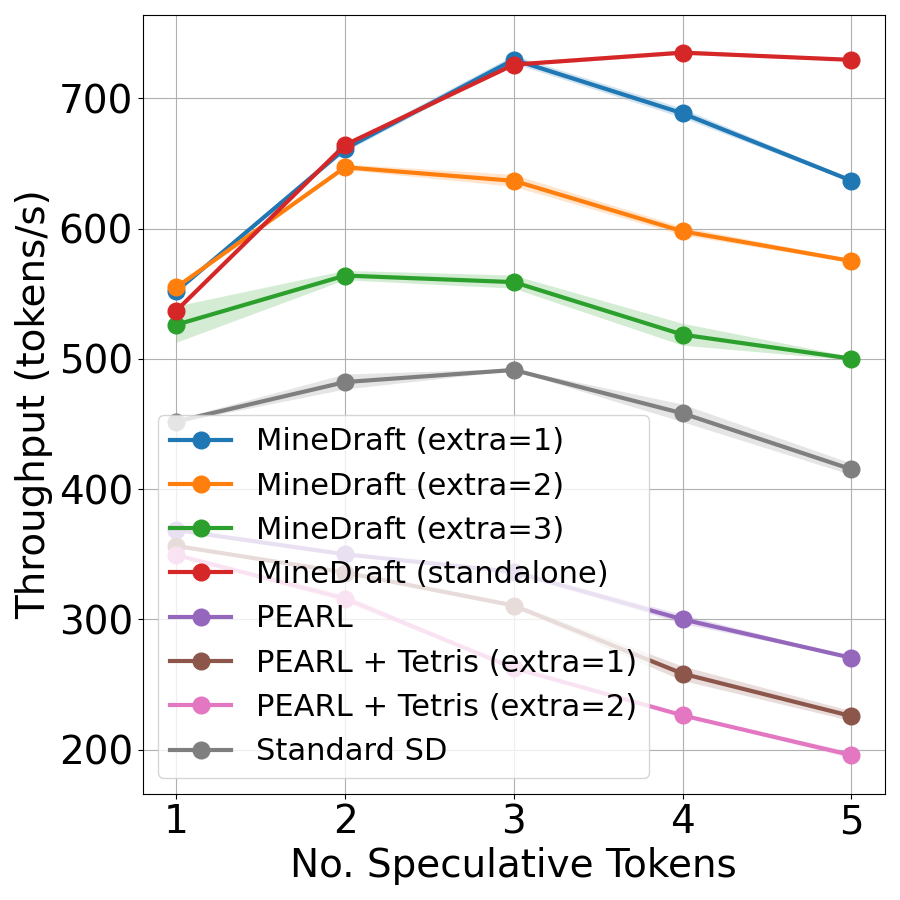
\includegraphics[width=0.23\linewidth]{results/Tough_Qwen3-32B_Qwen3-1_7B_1000_bs16_100pct_gen_throughput.png} \\
        & (a) \hspace{2mm} $\uparrow$ 38.62\%, $\Delta$ 69.19\% &
        (b) \hspace{2mm} $\uparrow$ 47.35\%, $\Delta$ 62.36\% &
        (c) \hspace{2mm} $\uparrow$ 40.90\%, $\Delta$ 62.80\% &
        (d) \hspace{2mm} $\uparrow$ 48.47\%, $\Delta$ 75.68\% \\

        \rotatebox{90}{\parbox{3.5cm}{\centering \hspace{8mm}\textbf{Qwen3~32B-4B}}} &
        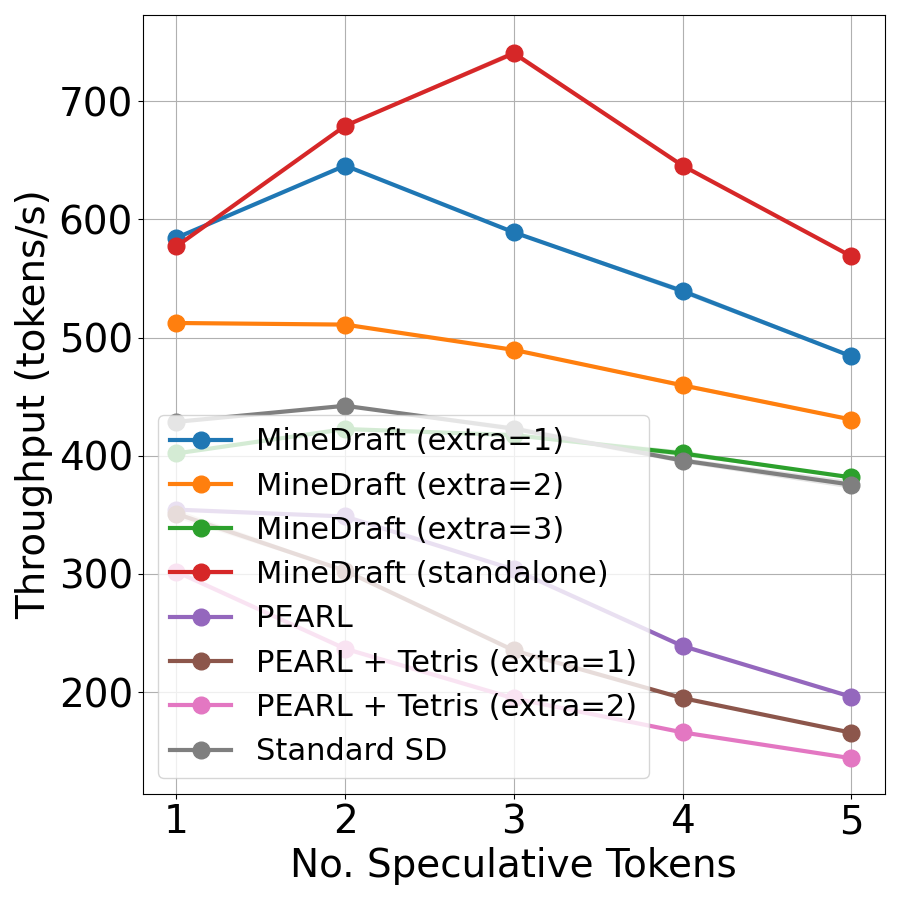
\includegraphics[width=0.23\linewidth]{results/Arena_Qwen3-32B_Qwen3-4B_1000_bs16_100pct_gen_throughput.png} &
        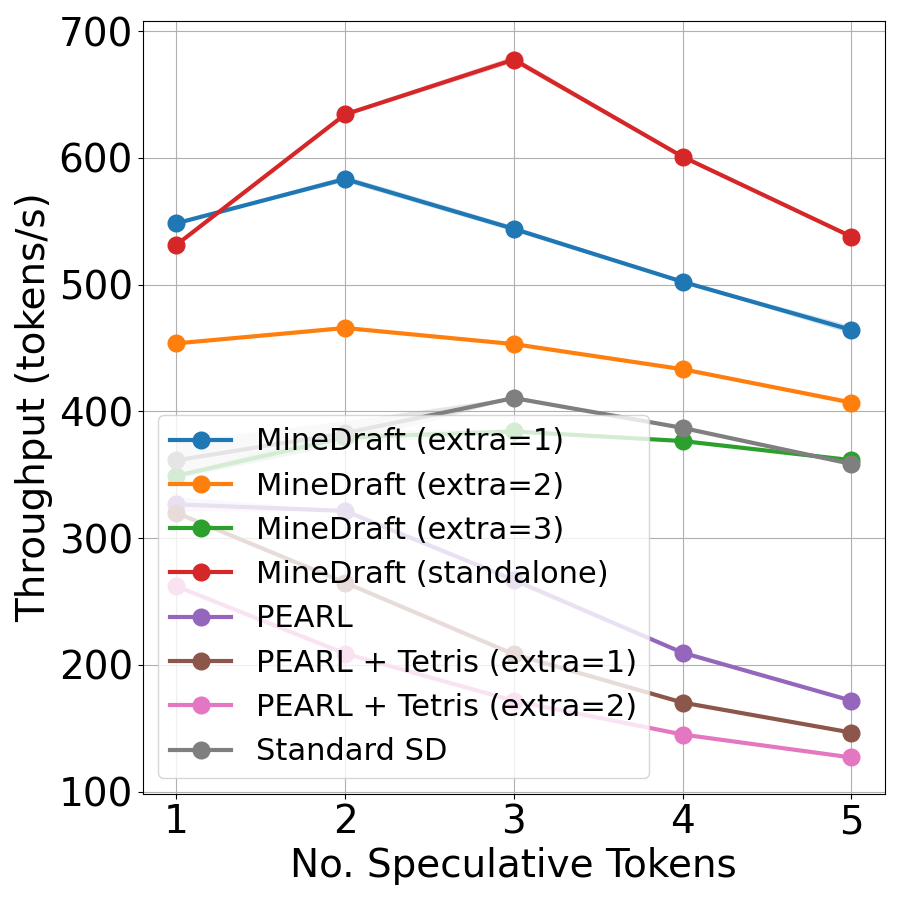
\includegraphics[width=0.23\linewidth]{results/ShareGPT_Qwen3-32B_Qwen3-4B_1000_bs16_100pct_gen_throughput.png} &
        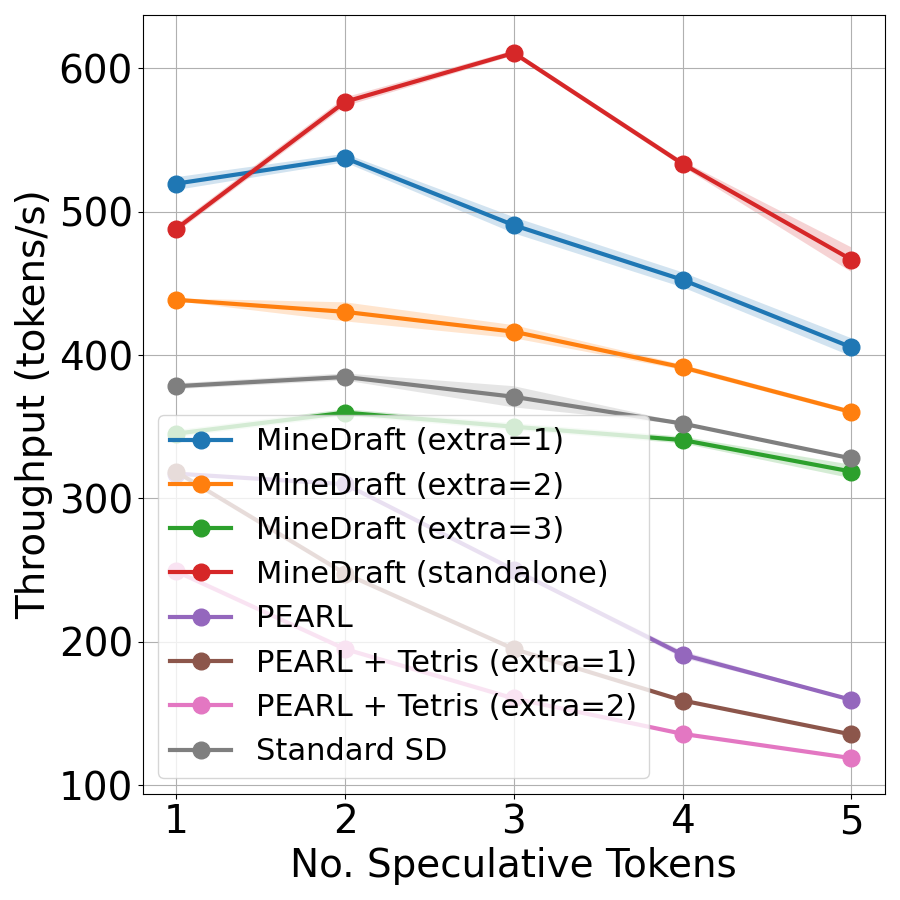
\includegraphics[width=0.23\linewidth]{results/Spec-Bench_Qwen3-32B_Qwen3-4B_161_bs16_100pct_gen_throughput.png} &
        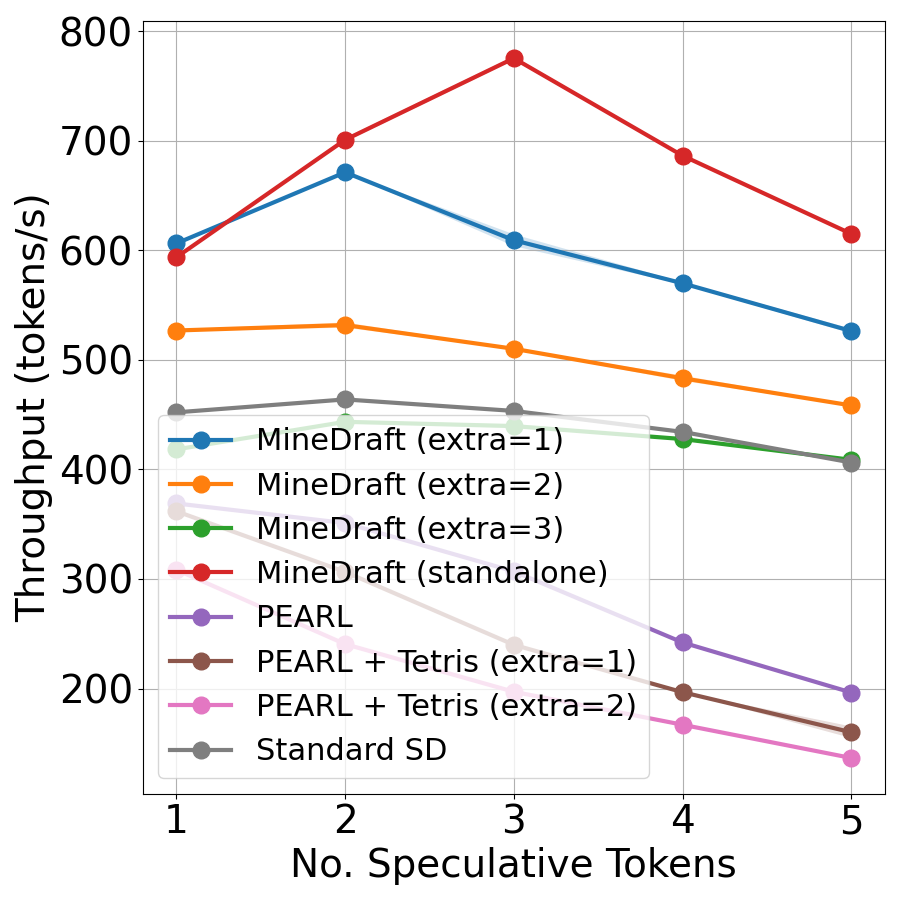
\includegraphics[width=0.23\linewidth]{results/Tough_Qwen3-32B_Qwen3-4B_1000_bs16_100pct_gen_throughput.png} \\
        & \hspace{2mm}(e) \hspace{2mm} $\uparrow$ 53.55\%, $\Delta$ 75.12\% &
        \hspace{2mm}(f) \hspace{2mm} $\uparrow$ 65.02\%, $\Delta$ 65.64\% &
        \hspace{2mm}(g) \hspace{2mm} $\uparrow$ 49.88\%, $\Delta$ 64.65\% &
        \hspace{2mm}(h) \hspace{2mm} $\uparrow$ 51.06\%, $\Delta$ 70.98\% \\
    \end{tabular}}
    \caption{
        Throughput comparison against baseline methods across model settings 1--3. $\uparrow$ indicates the average improvement over the best baseline method. $\Delta$ indicates the maximum average gap between \alg{} and standard SD. More details about $\uparrow$ and $\Delta$ are provided in \cref{app:performance_improvement}. 
        \alg{} consistently outperforms baselines, improving average throughput by up to 65.02\% over the best-performing baseline and by up to 75.68\% over standard SD.
    }
    \label{fig:throughput-baseline}
    \vspace{-4mm}
\end{figure*}

\begin{figure*}[!ht]
    \centering
    \setlength{\tabcolsep}{1pt} 
    \resizebox{0.99\linewidth}{!}{
    \begin{tabular}{ccccc}
        & \hspace{8mm}\textbf{Arena} & \hspace{8mm}\textbf{ShareGPT} & \hspace{8mm}\textbf{Spec-Bench}  & \hspace{8mm}\textbf{Tough}\\

        \rotatebox{90}{\parbox{3.5cm}{\centering \hspace{8mm}\textbf{Llama-3~70B-8B}}} & 
        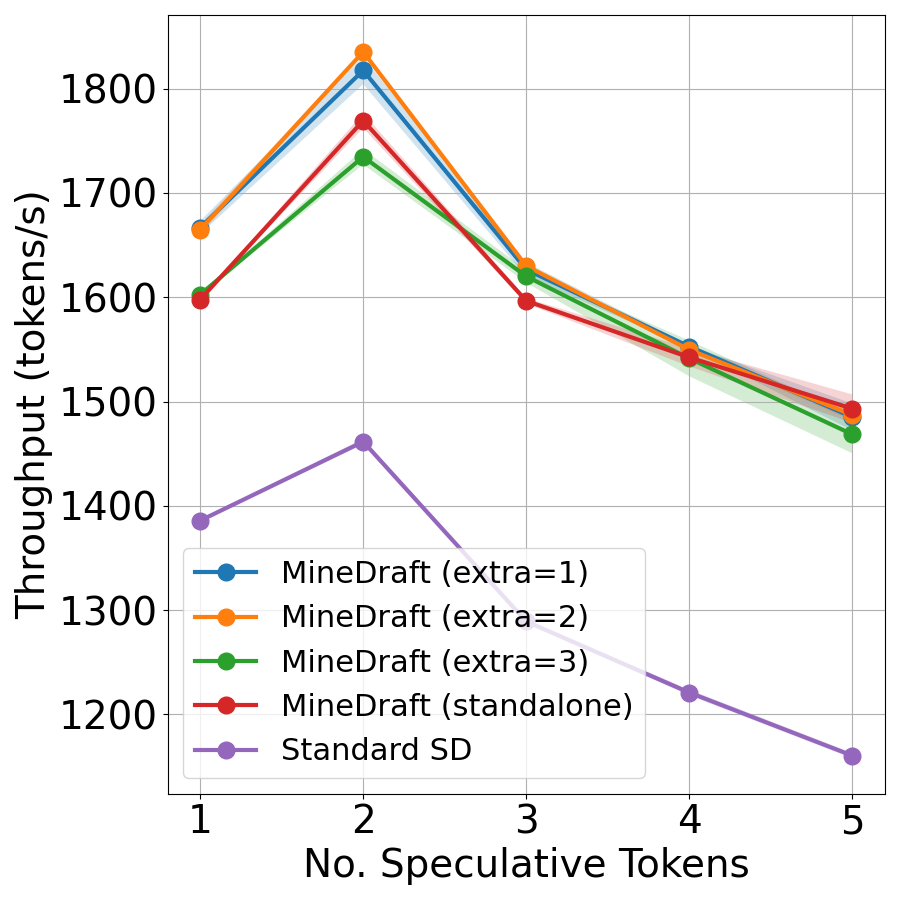
\includegraphics[width=0.23\linewidth]{results/Arena_Meta-Llama-3_3-70B-Instruct-AWQ-INT4_Llama-3_1-8B-Instruct_1000_bs64_100pct_gen_throughput.png} &
        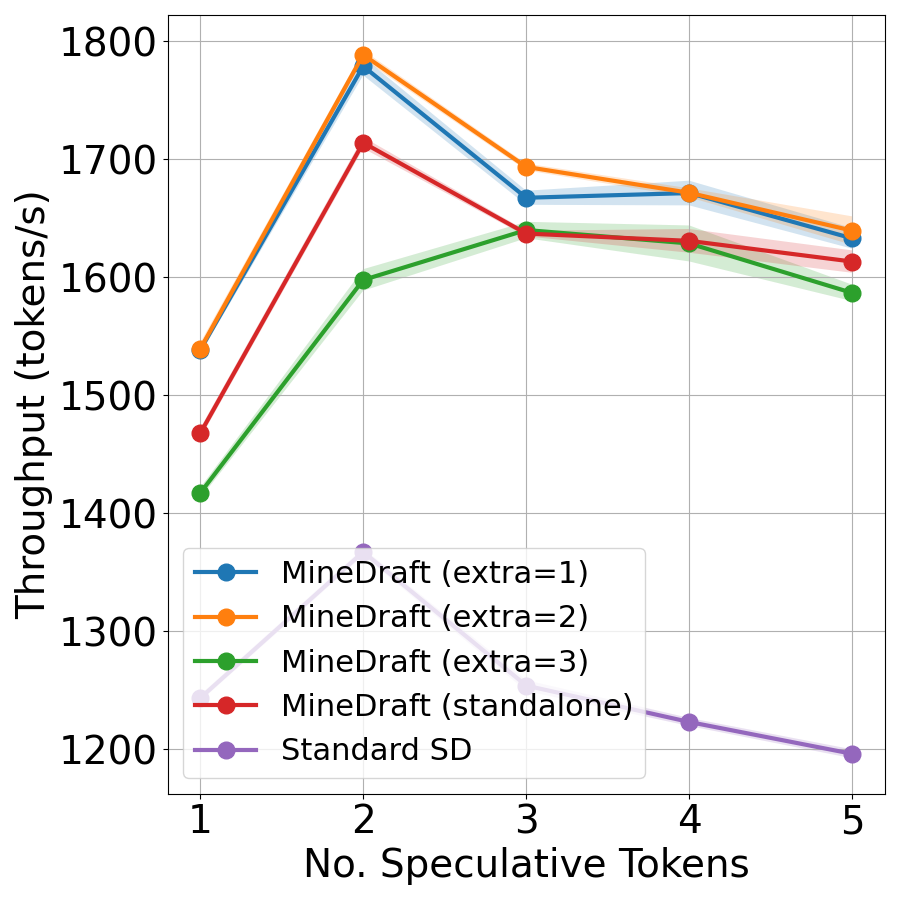
\includegraphics[width=0.23\linewidth]{results/ShareGPT_Meta-Llama-3_3-70B-Instruct-AWQ-INT4_Llama-3_1-8B-Instruct_1000_bs64_100pct_gen_throughput.png} &
        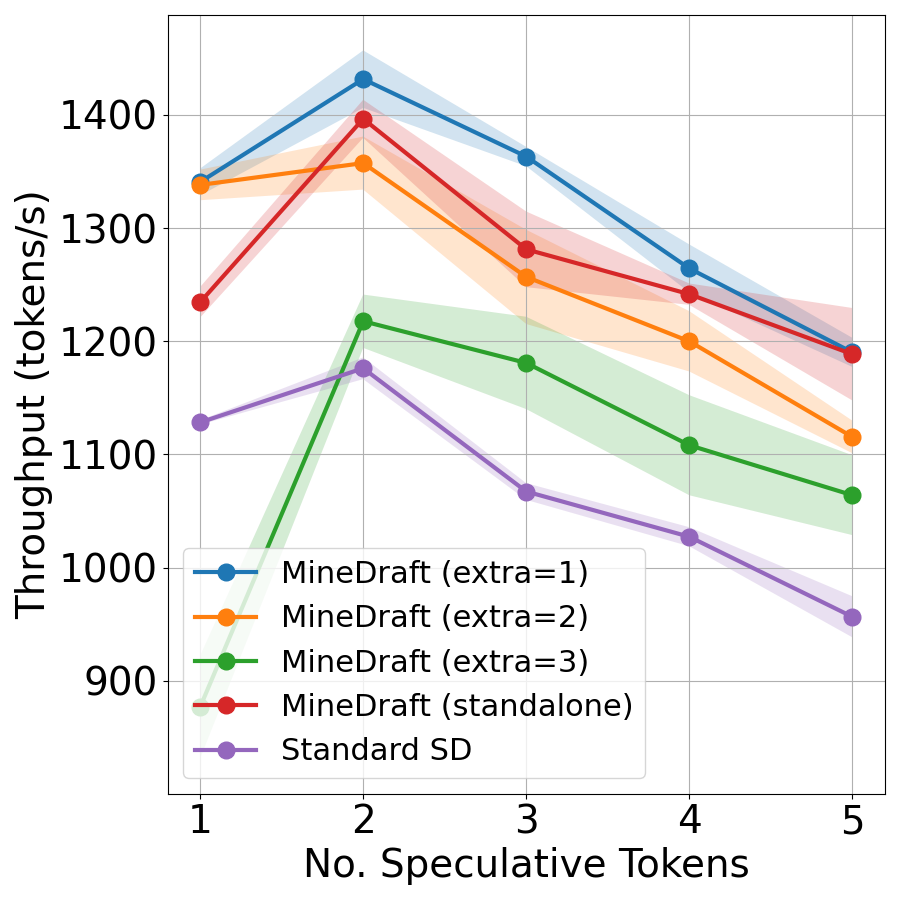
\includegraphics[width=0.23\linewidth]{results/Spec-Bench_Meta-Llama-3_3-70B-Instruct-AWQ-INT4_Llama-3_1-8B-Instruct_160_bs64_100pct_gen_throughput.png} &
        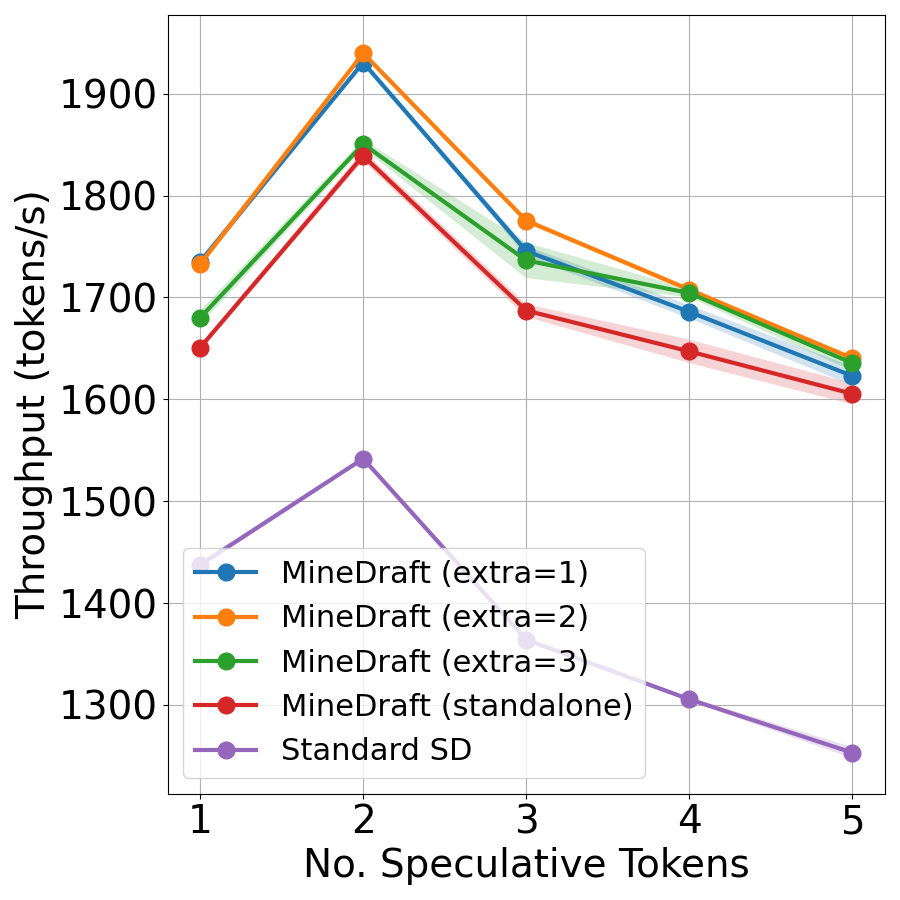
\includegraphics[width=0.23\linewidth]{results/Tough_Meta-Llama-3_3-70B-Instruct-AWQ-INT4_Llama-3_1-8B-Instruct_1000_bs64_100pct_gen_throughput.png} \\
        & (a) \hspace{2mm} $\uparrow$ 25.57\%, $\Delta$ 28.68\% &
        (b) \hspace{2mm} $\uparrow$ 30.81\%, $\Delta$ 37.06\% &
        (c) \hspace{2mm} $\uparrow$ 21.73\%, $\Delta$ 27.73\% &
        (d) \hspace{2mm} $\uparrow$ 25.81\%, $\Delta$ 30.89\% \\
        \vspace{2mm}
        \rotatebox{90}{\parbox{3.5cm}{\centering \hspace{8mm}\textbf{Vicuna~33B-EAGLE}}} &
        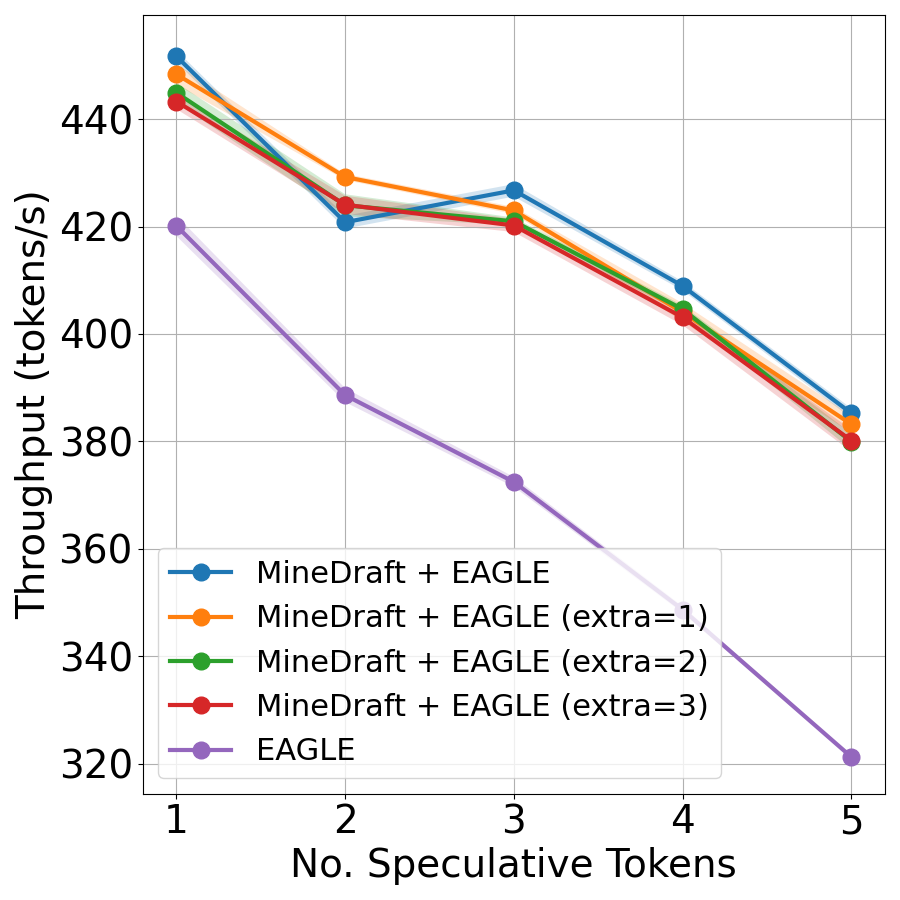
\includegraphics[width=0.23\linewidth]{results/Arena_vicuna-33b-v1_3_EAGLE-Vicuna-33B-v1_3_1000_bs16_100pct_gen_throughput.png} &
        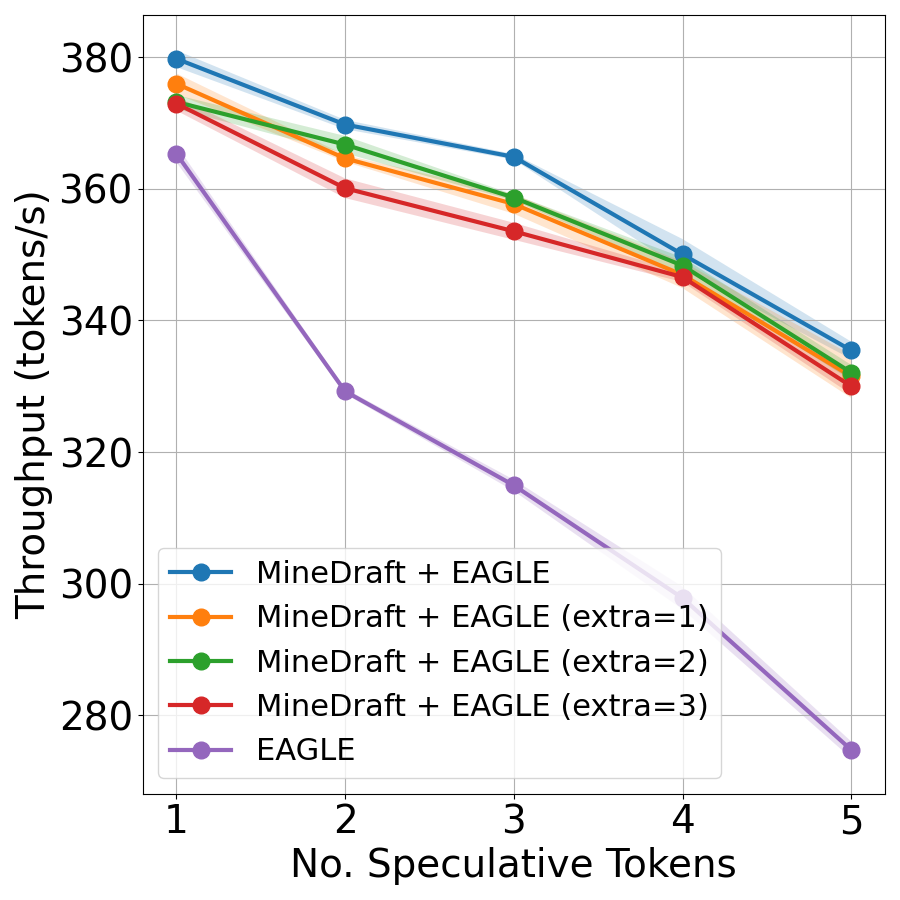
\includegraphics[width=0.23\linewidth]{results/ShareGPT_vicuna-33b-v1_3_EAGLE-Vicuna-33B-v1_3_1000_bs16_100pct_gen_throughput.png} &
        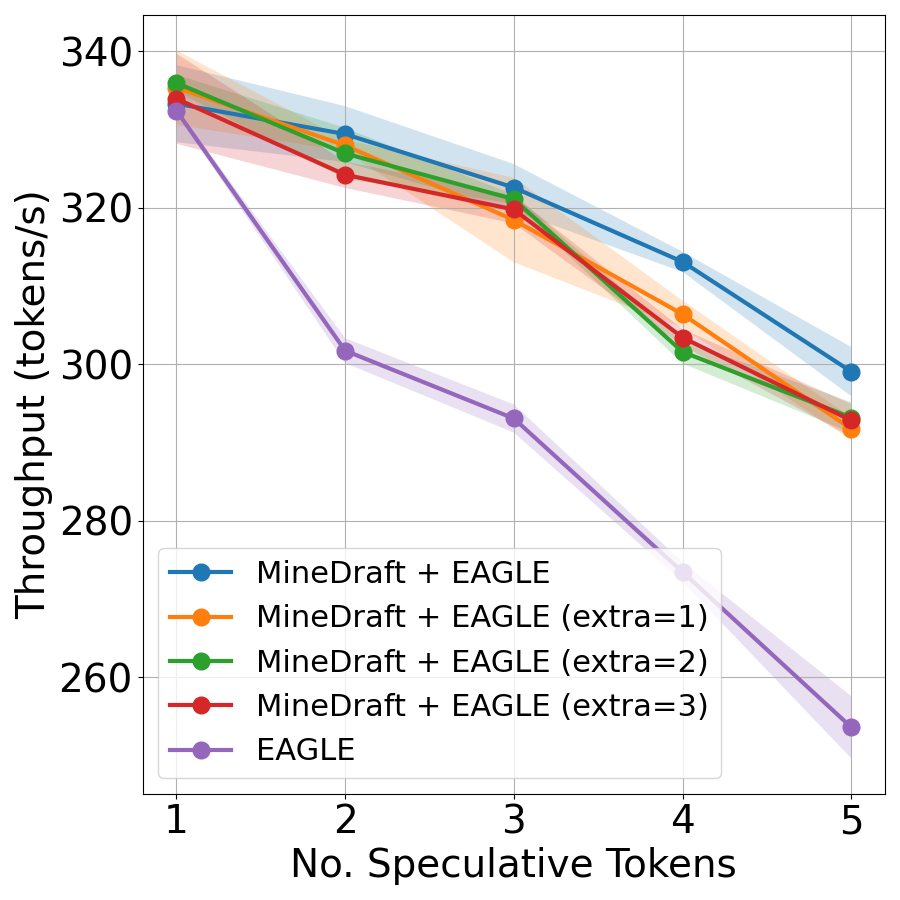
\includegraphics[width=0.23\linewidth]{results/Spec-Bench_vicuna-33b-v1_3_EAGLE-Vicuna-33B-v1_3_162_bs16_100pct_gen_throughput.png} &
        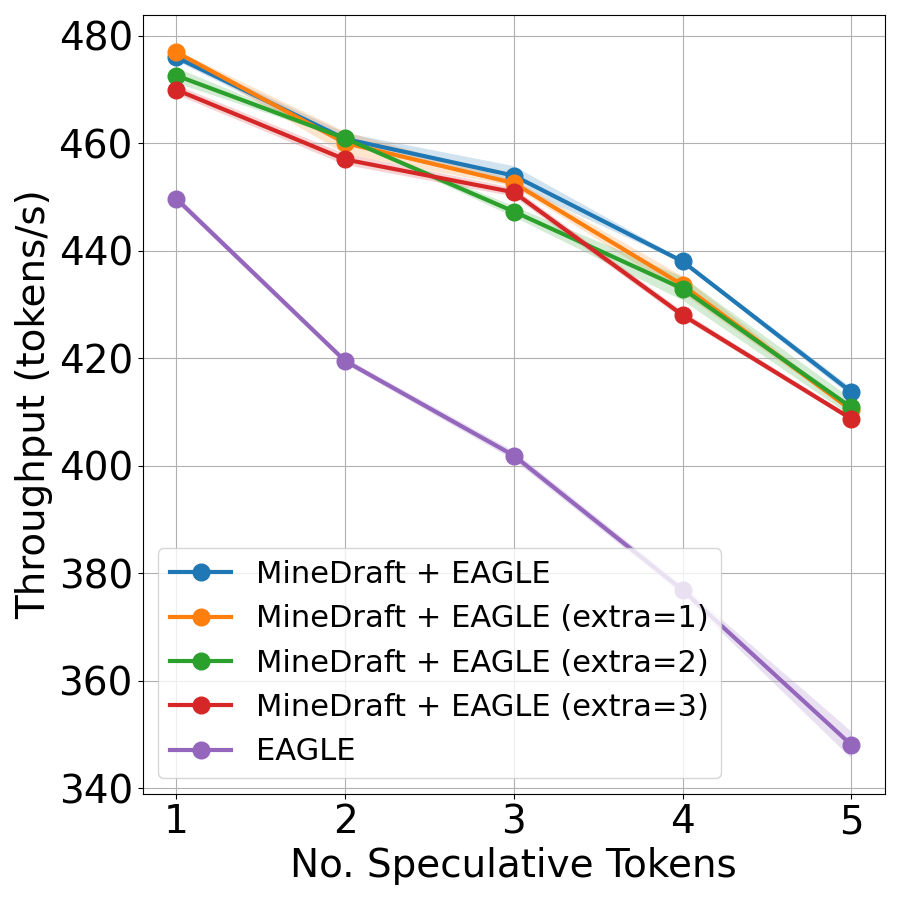
\includegraphics[width=0.23\linewidth]{results/Tough_vicuna-33b-v1_3_EAGLE-Vicuna-33B-v1_3_1000_bs16_100pct_gen_throughput.png} \\
        & \hspace{2mm}(e) \hspace{2mm} $\uparrow$ 7.51\%, $\Delta$ 19.91\% &
        \hspace{2mm}(f) \hspace{2mm} $\uparrow$ 3.95\%, $\Delta$ 22.09\% &
        \hspace{2mm}(g) \hspace{2mm} $\uparrow$ 1.06\%, $\Delta$ 17.92\% &
        \hspace{2mm}(h) \hspace{2mm} $\uparrow$ 6.06\%, $\Delta$ 18.87\% \\
    \end{tabular}}
    \caption{
        Throughput comparison across model settings 5 and 6. $\uparrow$ indicates the average improvement over the best baseline method. $\Delta$ indicates the maximum average gap between \alg{} and standard SD or EAGLE. 
        \alg{} consistently outperforms standalone EAGLE and standard SD, achieving maximum average throughput gains of 37.06\% and 22.09\%, respectively.
    }
    \label{fig:throughput-strategy}
\end{figure*}


\begin{figure*}[!ht]
    \centering
    \setlength{\tabcolsep}{1pt} 
    \resizebox{0.99\linewidth}{!}{
    \begin{tabular}{ccccc}
        & \hspace{8mm}\textbf{Arena} & \hspace{8mm}\textbf{ShareGPT} & \hspace{8mm}\textbf{Spec-Bench}  & \hspace{8mm}\textbf{Tough}\\

        \rotatebox{90}{\parbox{3.5cm}{\centering \hspace{8mm}\textbf{Qwen3~32B-8B}}} & 
        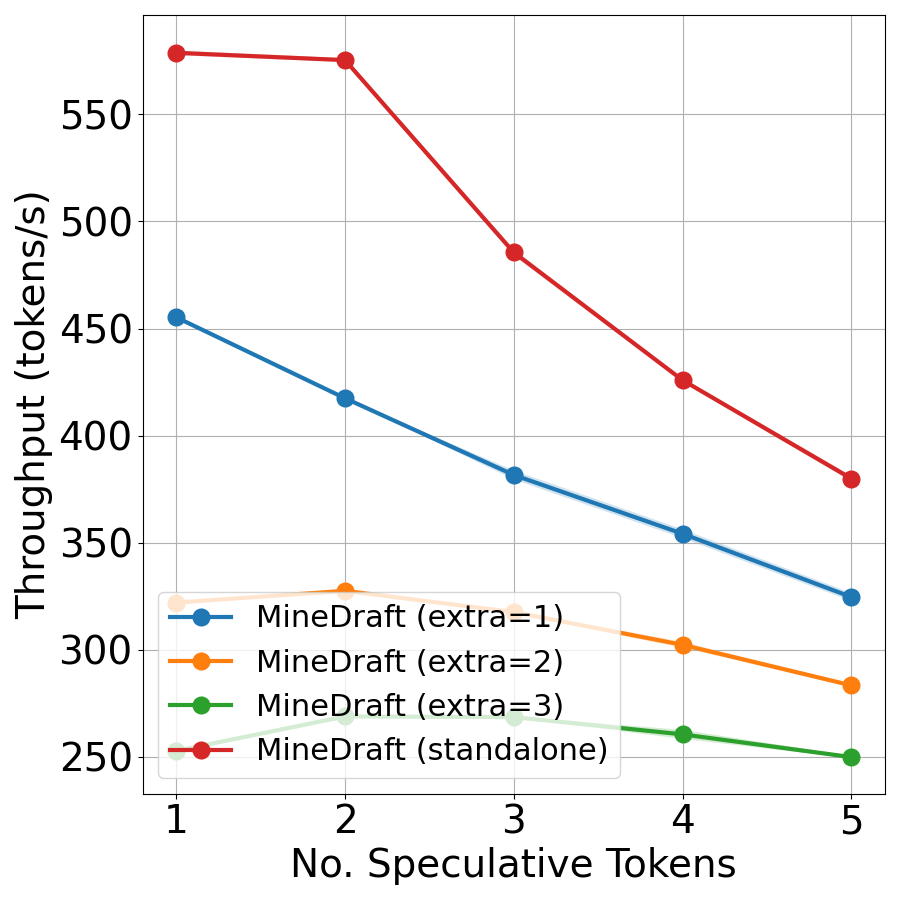
\includegraphics[width=0.23\linewidth]{results/Arena_Qwen3-32B_Qwen3-8B_1000_bs16_100pct_gen_throughput.png} &
        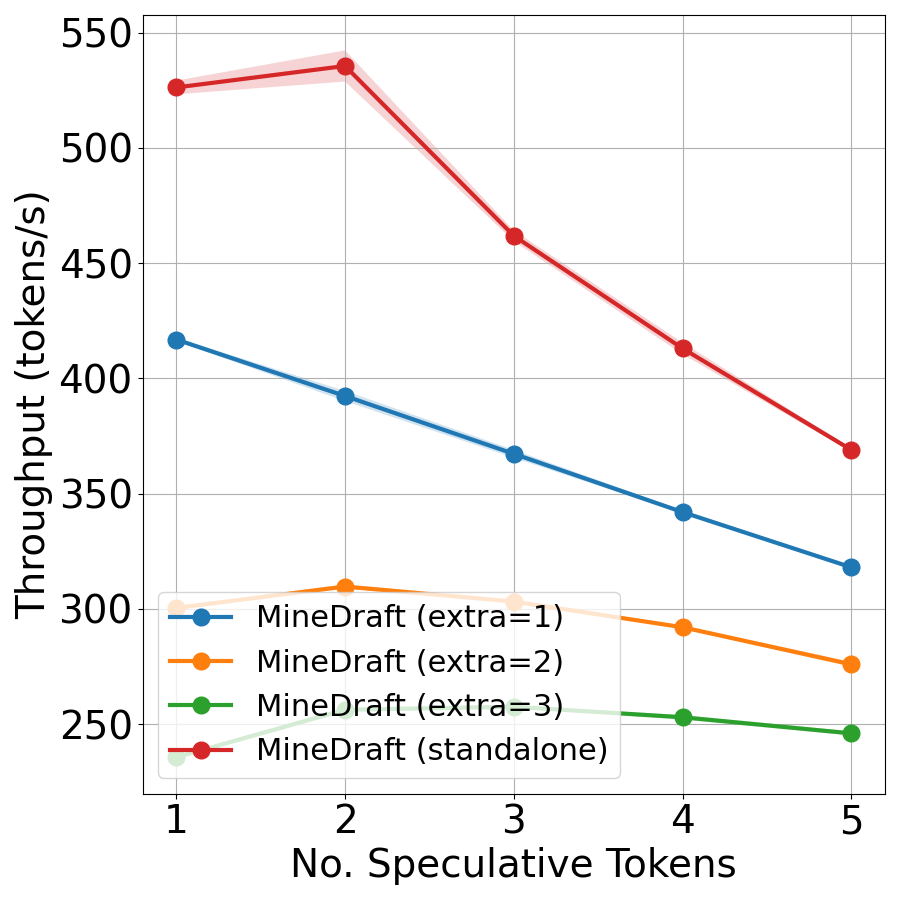
\includegraphics[width=0.23\linewidth]{results/ShareGPT_Qwen3-32B_Qwen3-8B_1000_bs16_100pct_gen_throughput.png} &
        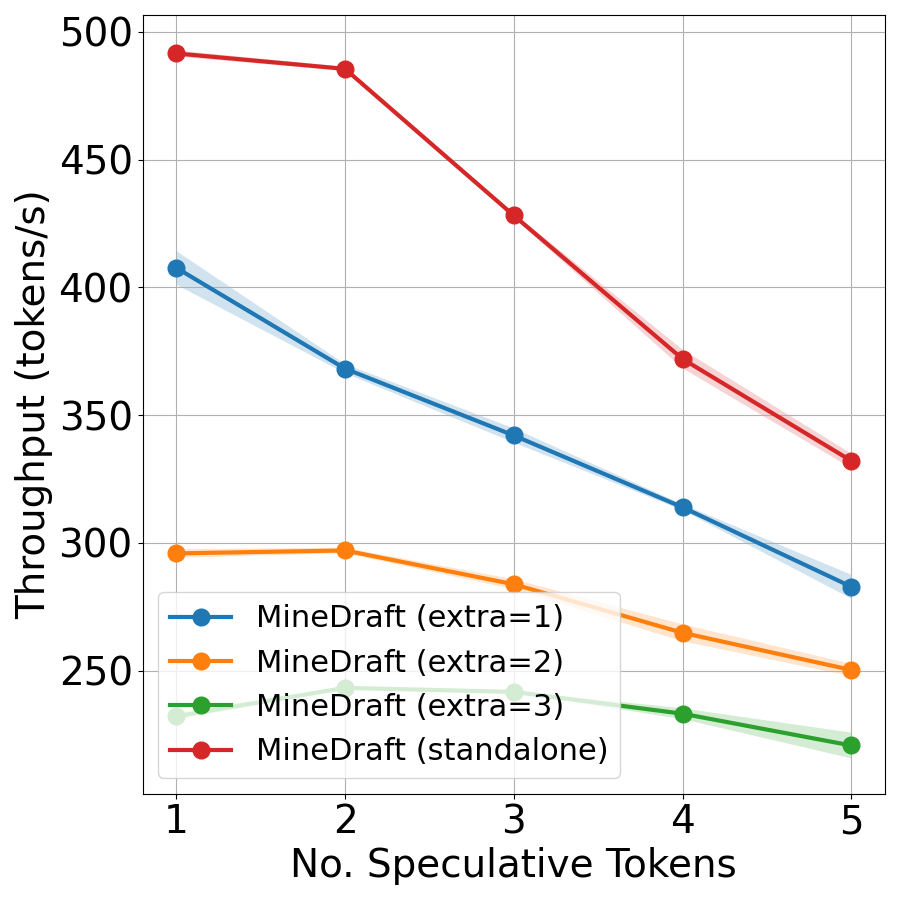
\includegraphics[width=0.23\linewidth]{results/Spec-Bench_Qwen3-32B_Qwen3-8B_161_bs16_100pct_gen_throughput.png} &
        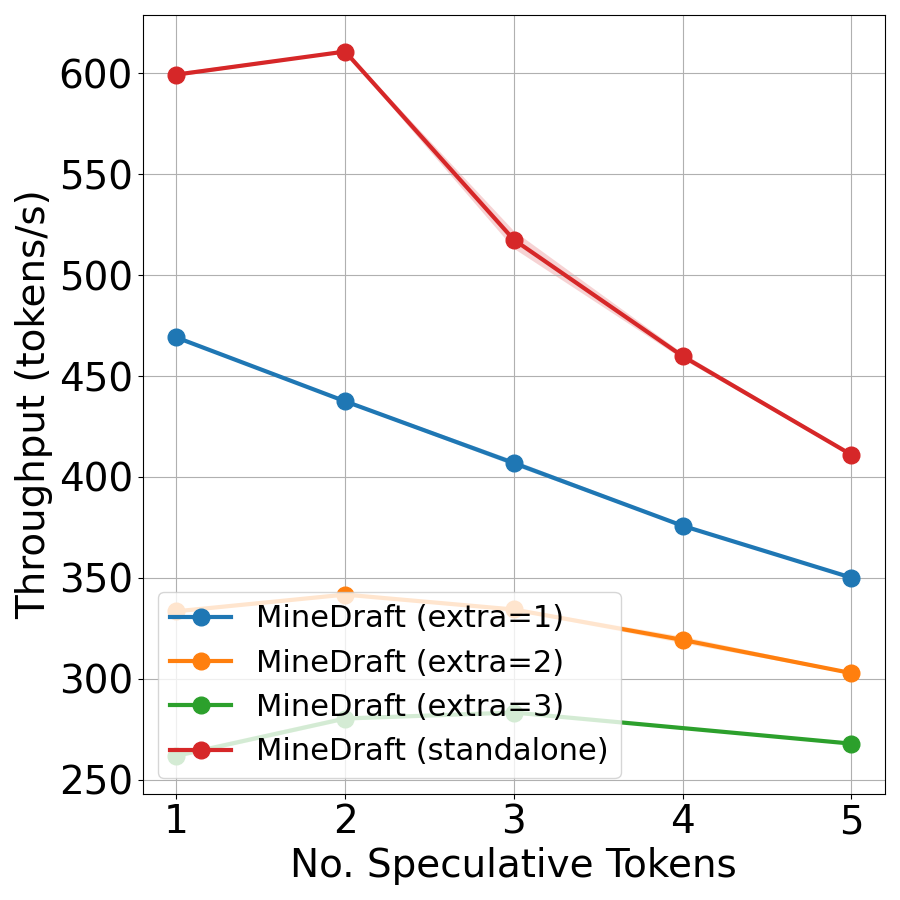
\includegraphics[width=0.23\linewidth]{results/Tough_Qwen3-32B_Qwen3-8B_1000_bs16_100pct_gen_throughput.png} \\

    \end{tabular}}
    \caption{
        Throughput results on model setting 4.
        Standard SD experiments failed on this setting due to OOM.
    }
    \label{fig:throughput-qwen8b}
\end{figure*}


\begin{figure*}[!ht]
    \centering
    \setlength{\tabcolsep}{1pt} 
    \resizebox{0.99\linewidth}{!}{
    \begin{tabular}{ccccc}
        & \hspace{8mm}\textbf{E2EL} & \hspace{8mm}\textbf{Different Draft Models} & \hspace{8mm}\textbf{Different \#Sequences}  & \hspace{8mm}\textbf{Different Batch Sizes}\\

        \rotatebox{90}{\parbox{3.5cm}{\centering \hspace{8mm}\textbf{Arena}}} & 
        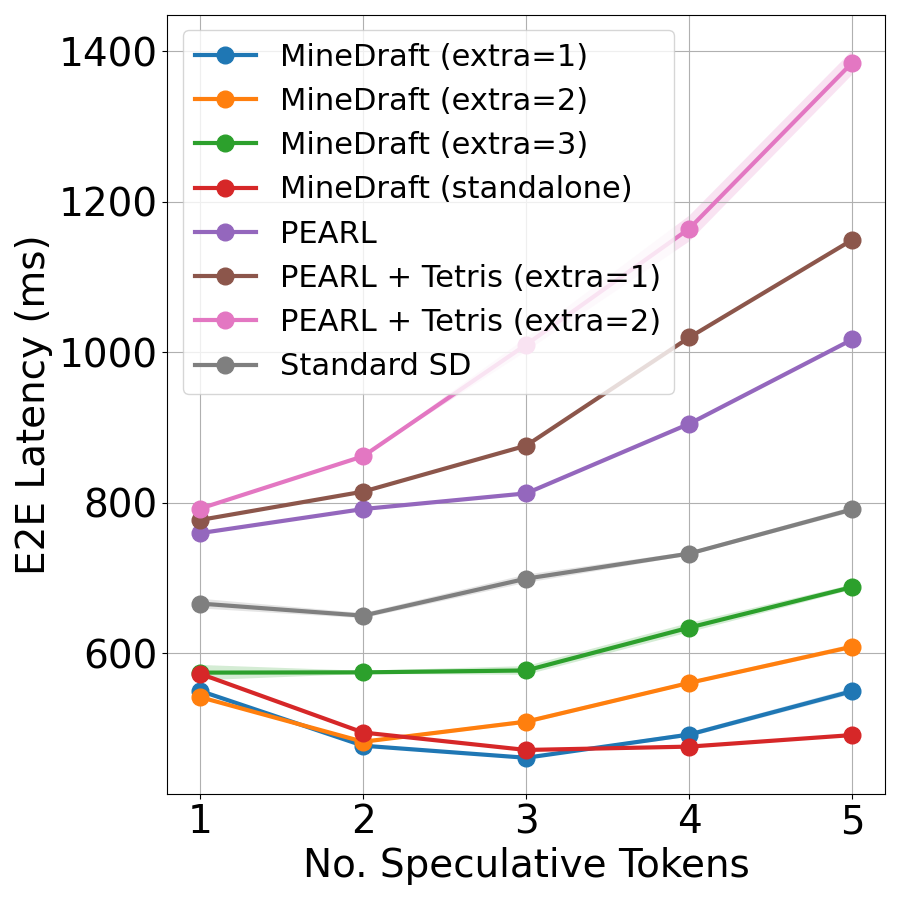
\includegraphics[width=0.23\linewidth]{results/Arena_Qwen3-32B_Qwen3-0_6B_1000_bs16_100pct_latency.png} &
        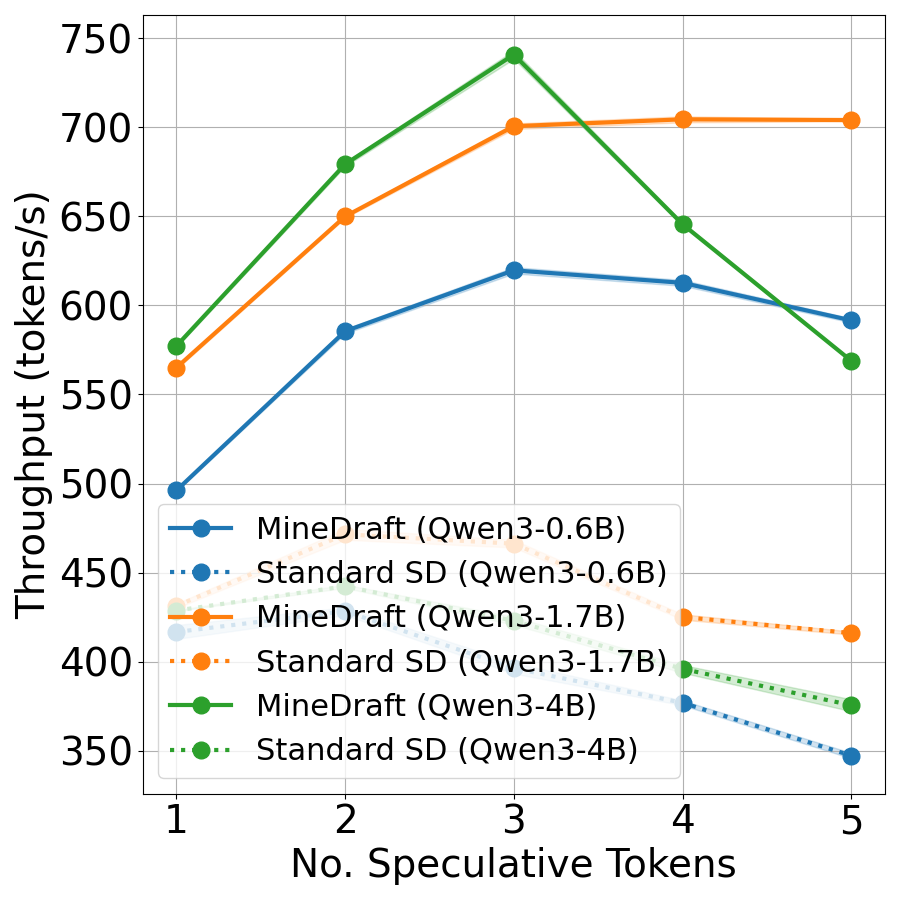
\includegraphics[width=0.23\linewidth]{results/Arena_Qwen3-32B_1000_bs16_100pct_gen_throughput.png} &
        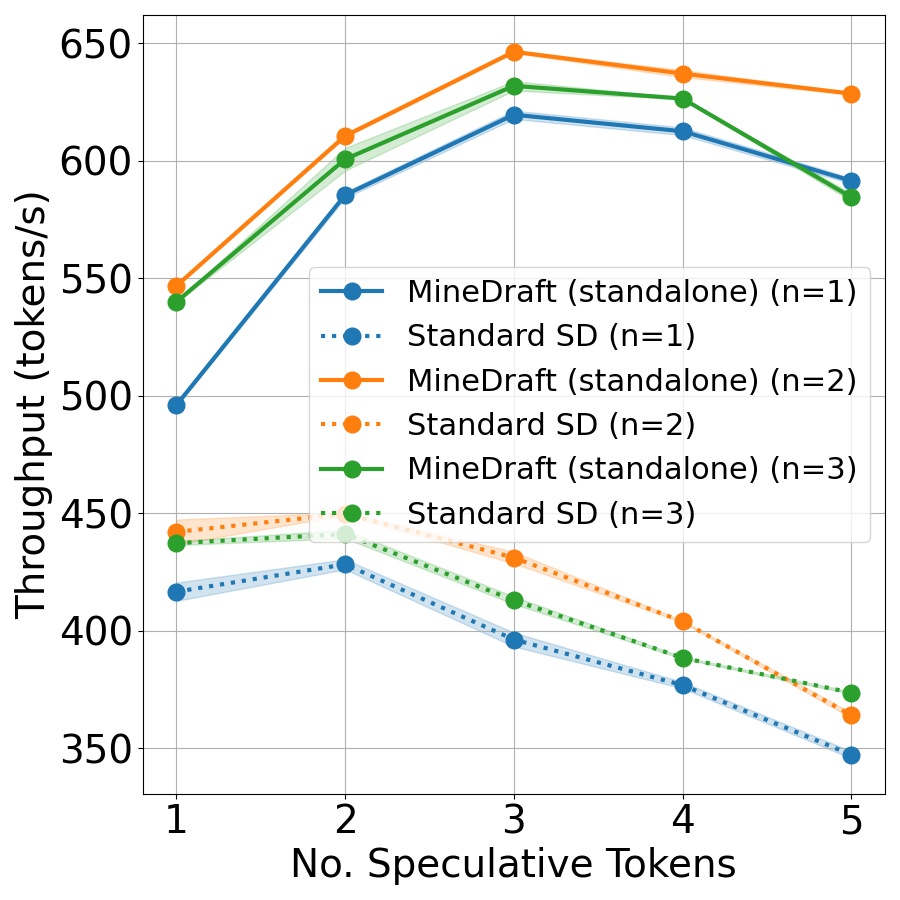
\includegraphics[width=0.23\linewidth]{results/Arena_Qwen3-32B_Qwen3-0_6B_1000_bs16_100pct_gen_throughput_vs_n.png} &
        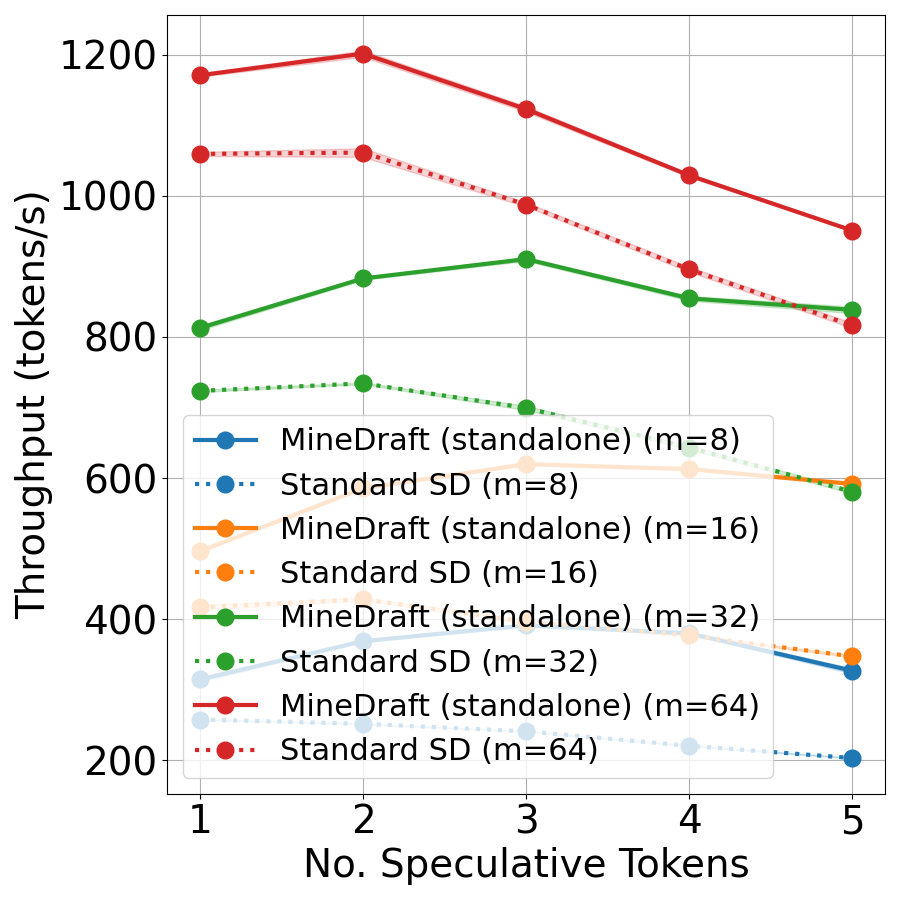
\includegraphics[width=0.23\linewidth]{results/Arena_Qwen3-32B_Qwen3-0_6B_1000_100pct_gen_throughput_vs_m.png} \\
        & \hspace{2mm}(a) &
        \hspace{2mm}(b) &
        \hspace{2mm}(c) &
        \hspace{2mm}(d) \\

    \end{tabular}}
    \caption{
        Different ablation studies using the Arena dataset.
        The comprehensive details and analysis of our ablation studies are included in \cref{app:exp-e2el,app:exp-draft-model,app:exp-n-m}. Plot (a) shows \alg{} consistently reduces end-to-end latency relative to baselines. Plot (b) indicates choice of draft model can affect \alg{}'s parallelism benefit. Plots (c) and (d) present how \alg{} scales with larger $n$ (number of sequences per request) and $m$ (batch size) values.
    }
    \label{fig:ablations}
\end{figure*}


We evaluate the effectiveness of \alg{} using the performance metrics introduced in \cref{sec:preliminaries}, namely average throughput (tokens/second or tokens/s) and end-to-end latency (milliseconds or ms). In addition to demonstrating the performance gains of \alg{}, our empirical results show that \alg{} can further improve speculative decoding by integrating existing drafting techniques.

% We evaluate the effectiveness of \alg{} on performance metrics introduced in \cref{sec:preliminaries}, specifically, average throughput (token/s) and end-to-end latency (ms). Apart from demonstrating the performance gain brought by \alg{}, we show that, with empirical results, the potential to further improve SD by integrating various existing techniques into \alg{}.

\para{Model settings.}
We consider seven target–draft model configurations, listed below. In all settings, the target model is served with tensor parallelism set to four, while a single GPU is dedicated to serving the draft model. Additional setup details are provided in \cref{app:exp-setup}.
\squishlisttwo
    \item \textbf{Settings 1--4} use Qwen3-32B~\citep{qwen3technicalreport} as the target model with different draft models: Qwen3-0.6B (Setting~1), Qwen3-1.7B (Setting~2), Qwen3-4B (Setting~3), Qwen3-8B (Setting~4). All are served on $5$ L40 GPUs with $m=16$.
    
    \item \textbf{Setting 5} pairs Llama-3.3-70B-Instruct-AWQ-INT4~\citep{llama3370bawq2024} as the target model with Llama-3.1-8B-Instruct~\citep{grattafiori2024llama3} as the draft model, served on five H100 GPUs with $m=64$.
    
    \item \textbf{Settings 6 and 7} use vicuna-33b-v1.3 and vicuna-13b-v1.3~\citep{zheng2023arena} as the target models, respectively, paired with EAGLE-Vicuna-33B-v1.3 and EAGLE-Vicuna-33B-v1.3~\citep{li2024eagle} as the draft model, respectively. These settings are served on five L40 GPUs with $m=16$.
\squishend


\para{Datasets.}
Following the experimental settings of prior work~\citep{hou2025banditspec,oliaro2025suffixdecoding,wu2025tetris}, we evaluate \alg{} on ShareGPT~\citep{sharegpt-dataset} (Apache License 2.0), Arena~\citep{zheng2023arena} (CC), LLM-Tough-Questions (Tough)~\citep{yav-ai2024domain-tough} (MIT License), and Spec-Bench~\citep{xia2024sd-survey} (Apache License 2.0), to robustly assess the applicability of \alg{} across a diverse range of scenarios.


\subsection{Comparison against Baselines.}
\label{subsec:exp-baseline}
We measure the average throughput of \alg{} and established baselines, including PEARL~\citep{liu2025pearl} and standard SD. As shown in \cref{fig:throughput-baseline}, \alg{} improves average throughput over the best-performing baseline by 38.62\% to 65.02\%, with maximum gains over standard SD ranging from 57.95\% to 75.68\%. 
These results show \alg{} consistently outperforms all baselines across all model settings and datasets.
For all experimental results, we report the mean and standard deviation over three independent trials unless otherwise specified.
We omit PEARL from subsequent experiments, as it exhibits substantially lower efficiency than \alg{} in preceding evaluations.


\para{Issue with extreme $k$ value.}
Notably, increasing the number of draft tokens per step is not always beneficial: excessive drafting can cause the draft stage to dominate verification time, thereby negating the benefit of hiding drafting latency via PSD. This effect is particularly significant for large draft models and is further analyzed in \cref{app:exp-draft-model}.


\subsection{Results with Different Drafting Strategies}
\label{ssec:Drafting_Strategies}
We further evaluate \alg{} integrated with other drafting strategies, including EAGLE and TETRIS, on the other model settings. As shown in \cref{fig:throughput-strategy}, integrating \alg{} with TETRIS and/or EAGLE consistently outperforms standalone EAGLE and standard SD across all datasets. In particular, \alg{} improves average throughput by up to 30.81\% and 7.51\% over the best results of standard SD and EAGLE, respectively. The maximum average improvements over standard SD and EAGLE reach 37.06\% and 22.09\%, respectively.

\para{Memory contention in standard SD.}
As shown in \cref{fig:throughput-qwen8b}, standard SD can encounter memory limitations when deploying larger draft models, such as Qwen3-8B, due to the coexistence of the draft and target models within the same GPU memory, which leads to VRAM contention. In contrast, the \alg{} architecture places the draft model on a dedicated GPU, enabling parallel drafting without competing for memory with the target model. This design alleviates memory bottlenecks and promotes a more balanced utilization of available GPU resources. Similar memory constraints arise for standard SD when deploying large target models, such as Qwen3-235B-A22B-Instruct-2507-FP8~\citep{qwen3technicalreport}, as detailed in \cref{app:exp-large-model}.


\para{EAGLE's subpar performance.} 
We observe that EAGLE’s performance degrades as the number of draft tokens per step increases, potentially due to the current vLLM implementation of EAGLE-based speculators, which is under investigation by the vLLM team~\citep{vllm_eagle_issue}.


\para{\alg{}'s as a batch PSD framework.} 
When integrated with TETRIS (denoted by ``extra='' in the legends), \alg{} outperforms its standalone variant under certain settings, highlighting its potential for further inference optimization when paired with effective drafting strategies. A more detailed breakdown of performance differences between integrations with drafting strategies and the standalone \alg{} implementation is left for future work.


\subsection{Ablation Studies}
\label{subsec:ablations}
This section presents representative ablation studies on the Arena dataset. Comprehensive results across all selected datasets are provided in \cref{app:exp-e2el,app:exp-draft-model,app:exp-n-m}. Due to space constraints, analysis of verification success rate of integration with TETRIS and Nsight Systems profiling results are also provided in \cref{sec:appendix}.


\para{End-to-end latency.}
We measure end-to-end latency of \alg{} and baseline methods under various drafting strategies across the model settings and datasets as described above. \cref{fig:ablations} shows representative results for Setting~1 on the Arena dataset, where \alg{} achieves a 26.58\% latency reduction relative to the best-performing baseline and a maximum reduction of 37.89\% compared to standard SD. A complete results are provided in \cref{app:exp-e2el}.


\para{Draft model sizes.}
We study the impact of draft model scale on system performance. Although \alg{} consistently outperforms standard SD across draft model sizes, \cref{fig:ablations} shows that increasing the number of draft tokens per step does not monotonically improve average throughput. This degradation is most pronounced for Qwen3-4B: when more than three draft tokens are generated per step, throughput drops below that achieved with only two draft tokens. A detailed analysis of this behavior is provided in \cref{app:exp-draft-model}.


\para{Scaling behavior with $n$ and $m$.}
We evaluate throughput scaling with respect to the number of sequences per request ($n$) and batch size ($m$). The final two plots in \cref{fig:ablations} show that, with $m$ held constant, increasing $n$ yields only marginal throughput gains, whereas increasing $m$ consistently improves average throughput. Moreover, when the number of draft tokens per step exceeds 4, the average throughput of \alg{} approaches that of standard SD with doubled batch size, suggesting that \alg{} can complement adaptive drafting strategies, which are often limited by draft length, to enable additional performance gains. More experiments are provided in \cref{app:exp-n-m}.